% !TeX root = RJwrapper.tex
\title{learningtower: an R package for Exploring Standardised Test
Scores Across the Globe}
\author{by Priya Ravindra Dingorkar, Kevin Y.X. Wang, and Dianne Cook}

\maketitle

\abstract{%
An abstract of less than 150 words - Discuss what the paper talks about
with a little introduction.
}

\hypertarget{introduction}{%
\section{Introduction}\label{introduction}}

The Organization for Economic Cooperation and Development
\href{OECD\%20-\%20https://www.oecd.org/about/}{OECD} is a global
organization that aims to create better policies for better lives. Its
mission is to create policies that promote prosperity, equality,
opportunity, and well-being for all.
\href{PISA\%20-\%20https://www.oecd.org/pisa/}{PISA} is one of OECD's
Programme for International Student Assessment. PISA assesses
15-year-old students' potential to apply their knowledge and abilities
in reading, mathematics, and science to real-world challenges. OECD
launched this in 1997, it was initially administered in 2000, and it
currently includes over
\href{https://www.oecd.org/pisa/aboutpisa/pisa-participants.htm}{80
nations}. The PISA study, conducted every three years, provides
comparative statistics on 15-year-olds' performance in reading, maths,
and science. This paper describes how to utilize the
\texttt{learningtower} package, which offers OECD PISA datasets from
2000 to 2018 in an easy-to-use format. This dataset comprises
information on their test results and other socioeconomic factors, as
well as information on their schools, infrastructure and the countries
participating in the program.

\hypertarget{what-is-pisa}{%
\section{What is PISA?}\label{what-is-pisa}}

PISA assesses the extent to which children approaching the end of
compulsory school have learned some of the information and abilities
required for full participation in modern society, notably in maths,
reading, and science. The examination focuses on reading, mathematics,
science, and problem solving. It also assesses students capacity to
replicate information and extrapolate from what they have learned and
apply that knowledge in unexpected circumstances, both inside and
outside of school. This approach reflects the fact that individuals are
rewarded in modern economies not for what they know, but for what they
can accomplish with what they know.

This evaluation which is carried out every three years, assists in
identifying students' development of knowledge and skills throughout the
world, which can provide actionable insights and therefore assist
education policymakers. PISA is well known for its distinctive testing
characteristics, which include policy orientation, an innovative notion
of literacy, relevance to lifelong learning, regularity, and breadth of
coverage. PISA is now used as an assessment tool in many regions around
the world. In addition to OECD member countries, the survey has been or
is being conducted in East, South and Southeast Asia, Central,
Mediterranean and Eastern Europe, and Central Asia, The Middle East,
Central and South America and Africa.

For each year of the PISA study, one domain subject is thoroughly
examined. In 2018, for example, reading was assessed alongside
mathematics and science as minor areas of assessment. The 2012 survey
concentrates on mathematics, with reading, science, and problem solving
serving as minor evaluation topics. PISA targets a certain age group of
students in order to properly compare their performance worldwide. PISA
students are aged between 15 years 3 months and 16 years 2 months at the
time of the assessment, and have completed at least 6 years of formal
schooling. They can enroll in any sort of institution, participate in
full-time or part-time education, academic or vocational programs, and
attend public, private, or international schools inside the country.
Using this age across nations and throughout time allows PISA to compare
the knowledge and abilities of people born in the same year who are
still in school at the age of 15, irrespective of their diverse
schooling.

The PISA test is primarily computer-based and lasts around 2 hours. The
examination comprises both multiple choice and free entry questions.
Some countries that were not ready for computer-based delivery carried
out the testing on paper. Each student may have a unique set of
questions. An example of the test may be seen
\href{https://www.oecd.org/pisa/test/}{here}. PISA assessment areas seek
to measure the following aspects of students' literacy in math, reading,
and science. The goal of mathematical literacy is to assess students
ability to grasp and interpret mathematics in a variety of settings.
Reading literacy assesses students' capacity to absorb, apply, analyze,
and reflect on texts in order to attain required goals and participate
in society. Science literacy is described as the ability to engage with
science-related issues and scientific concepts as a reflective citizen.

PISA data is publicly accessible for
\href{https://www.oecd.org/pisa/data/}{download}. Furthermore, reading
the
\href{https://www.oecd.org/pisa/data/pisa2018technicalreport/Ch.09-Scaling-PISA-Data.pdf}{data
documentation} reveals that the disclosed PISA scores are generated
using a sophisticated linear model applied to the data. For each
student, several values are simulated. This is known as synthetic data,
and it is a popular technique to ensuring data privacy. The data can
still be deemed accurate within the mean, variance, and stratum used in
the original data's modelling. In addition, the PISA website provides
the data in SPSS and SAS format, which can limit accessibility due to
the commercial nature of these software. Furthermore, all questions are
assigned with unique IDs within each year of the PISA study, but do not
always agree across the different years. This data has now been curated
and simplified into a single R package called \texttt{learningtower},
which contains all of the PISA scores from the years 2000 to 2018.

\hypertarget{data-compilation}{%
\section{Data Compilation}\label{data-compilation}}

Each developer at the ROpenSci OzUnconf was assigned to curate a
specific year of the PISA study. Data on the participating students and
schools were first downloaded from the PISA website, in either SPSS or
SAS format. The data were read into an R environment with the exception
of the year 2000 and 2003. Due to formatting issues, the data for these
two particular years were first read using SPSS and then exported into
compatible \texttt{.sav} files. After some data cleaning and wrangling
with the appropriate script, the variables of interest were
re-categorised and saved as RDS files. One major challenge faced by the
developers was to ensure the consistency of variables over the years.
For example, a student's mother's highest level of education was never
recorded in 2000, but it was categorised as ``ST11R01'' between 2003 and
2012 and ``ST005Q01TA'' between 2015 and 2018. Such a problem was
tackled manually by curating these values as an integer variable named
``mother\_educ'' in the output data. These final RDS file for each PISA
year were then thoroughly vetted and made available in a separate
\href{https://github.com/kevinwang09/learningtower_masonry}{GitHub
repository}.

\hypertarget{what-islearningtower}{%
\section{\texorpdfstring{What
is\texttt{learningtower}?}{What islearningtower?}}\label{what-islearningtower}}

\href{https://cran.r-project.org/web/packages/learningtower/index.html}{`learningtower'}
is an easy-to-use R package that provides quick access to a variety of
variables using OECD PISA data collected over a three-year period from
2000 to 2018. This dataset includes information on the PISA test scores
in mathematics, reading, and science. Furthermore, these datasets
include information on other socioeconomic aspects, as well as
information on their school and its facilities, as well as the nations
participating in the program.

The motivation for developing the \texttt{learningtower} package was
sparked by the announcement of the PISA 2018 results, which caused a
collective wringing of hands in the Australian press, with headlines
such as
\href{https://theconversation.com/vital-signs-australias-slipping-student-scores-will-lead-to-greater-income-inequality-128301}{``Vital
Signs: Australia's slipping student scores will lead to greater income
inequality''} and
\href{https://www.smh.com.au/education/in-china-nicholas-studied-maths-20-hours-a-week-in-australia-it-s-three-20191203-p53ggv.html}{``In
China, Nicholas studied maths 20 hours a week. In Australia, it's
three''}. That's when several academics from Australia, New Zealand, and
Indonesia decided to make things easier by providing easy access to PISA
scores as part of the \href{https://ozunconf19.ropensci.org/}{ROpenSci
OzUnconf}, which was held in Sydney from December 11 to 13, 2019. The
data from this survey, as well as all other surveys performed since the
initial collection in 2000, is freely accessible to the public. However,
downloading and curating data across multiple years of the PISA study
could be a time consuming task. As a result, we have made a more
convenient subset of the data freely available in a new R package called
\texttt{learningtower}, along with sample code for analysis.

The \texttt{learningtower} package primarily comprised of three
datasets: \texttt{student}, \texttt{school}, and \texttt{countrycode.}
The \texttt{student} dataset includes results from triennial testing of
15-year-old students throughout the world. This dataset also includes
information about their parents' education, family wealth, gender, and
presence of computers, internet, vehicles, books, rooms, desks, and
other comparable factors. Due to the size limitation on CRAN packages,
only a subset of the student data can be made available in the
downloaded package. These subsets of the student data, known as the
\texttt{student\_subset\_yyyy} (\texttt{yyyy} being the specific year of
the study) allow uses to quickly load, visualise the trends in the full
data. The full student dataset can be downloaded using the
\texttt{load\_student()} function included in this
\href{https://kevinwang09.github.io/learningtower/}{package.} The
\texttt{school} dataset includes school weight as well as other
information such as school funding distribution, whether the school is
private or public, enrollment of boys and girls, school size, and
similar other characteristics of interest of different schools these
15-year-olds attend around the world. The \texttt{countrycode} dataset
includes a mapping of a country/region's ISO code to its full name.

\texttt{learningtower} developers are committed to providing R users
with data to analyse PISA results every three years. Our package's
future enhancements include updating the package every time additional
PISA scores are announced. Note that, in order to account for post
COVID-19 problems, OECD member nations and associates decided to
postpone the PISA 2021 evaluation to 2022 and the PISA 2024 assessment
to 2025.

\hypertarget{example-analysis}{%
\section{Example Analysis}\label{example-analysis}}

In this section we will illustrate how the \texttt{learningtower}
package can be utilized to answer some research questions by applying
various methodologies and statistical computations on the
\texttt{learningtower} datasets.

We will use only the 2018 data here for illustrative purpose. We will
begin first by constructing a \texttt{data.frame} that records the
(weighted) average maths score for each country/region, grouped by
gender. We will also calculate the difference between the two averages
by gender. In order to show the variability in the mean estimate, we
will perform sampling with replace on the data and calculate the same
mean difference estimate. The empirical 90\% confidence intervals are
shown for each estimate for each country. We will repeat this process
for reading and science test scores.

\hypertarget{gender-analysis}{%
\section{Gender Analysis}\label{gender-analysis}}

\begin{Schunk}
\begin{figure}[H]
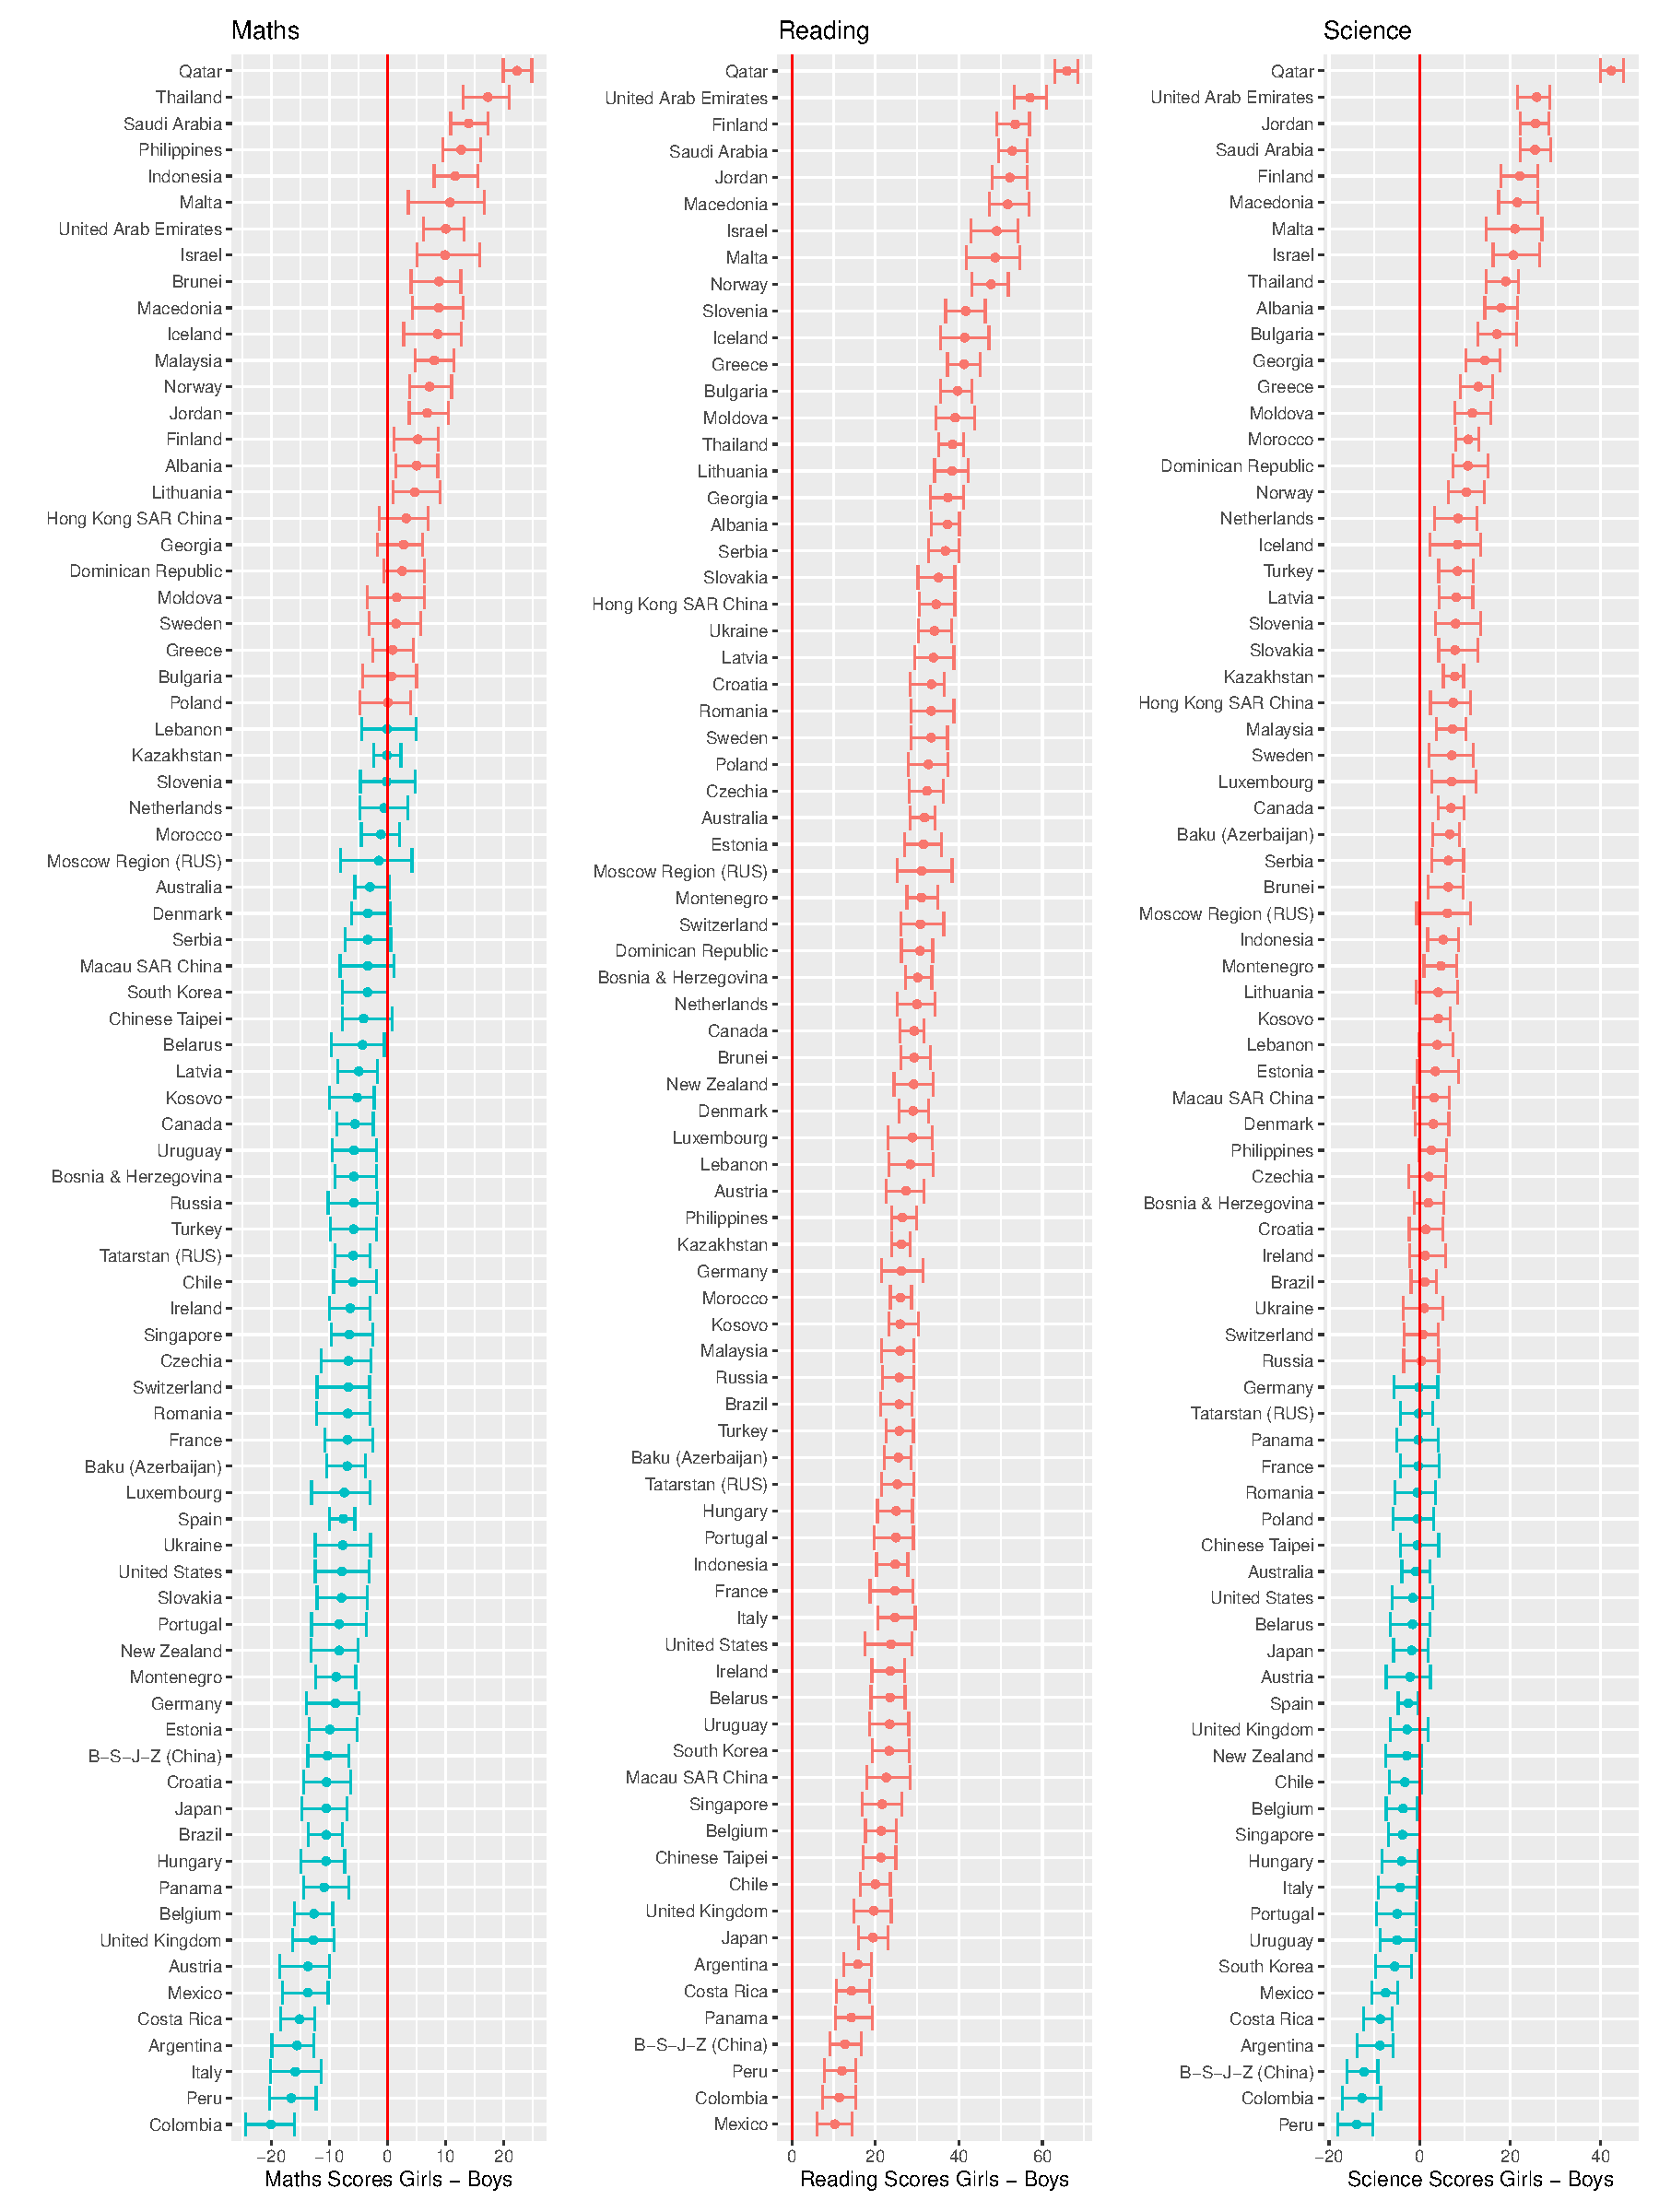
\includegraphics[width=1\linewidth]{learningtower_files/figure-latex/score-differences-1} \caption[Gender Analysis]{Gender Analysis}\label{fig:score-differences}
\end{figure}
\end{Schunk}

Figure \ref{fig:score-differences} shows differences between mean scores
for the three topics.

\hypertarget{maps}{%
\section{Maps}\label{maps}}

\begin{Schunk}
\begin{figure}[H]
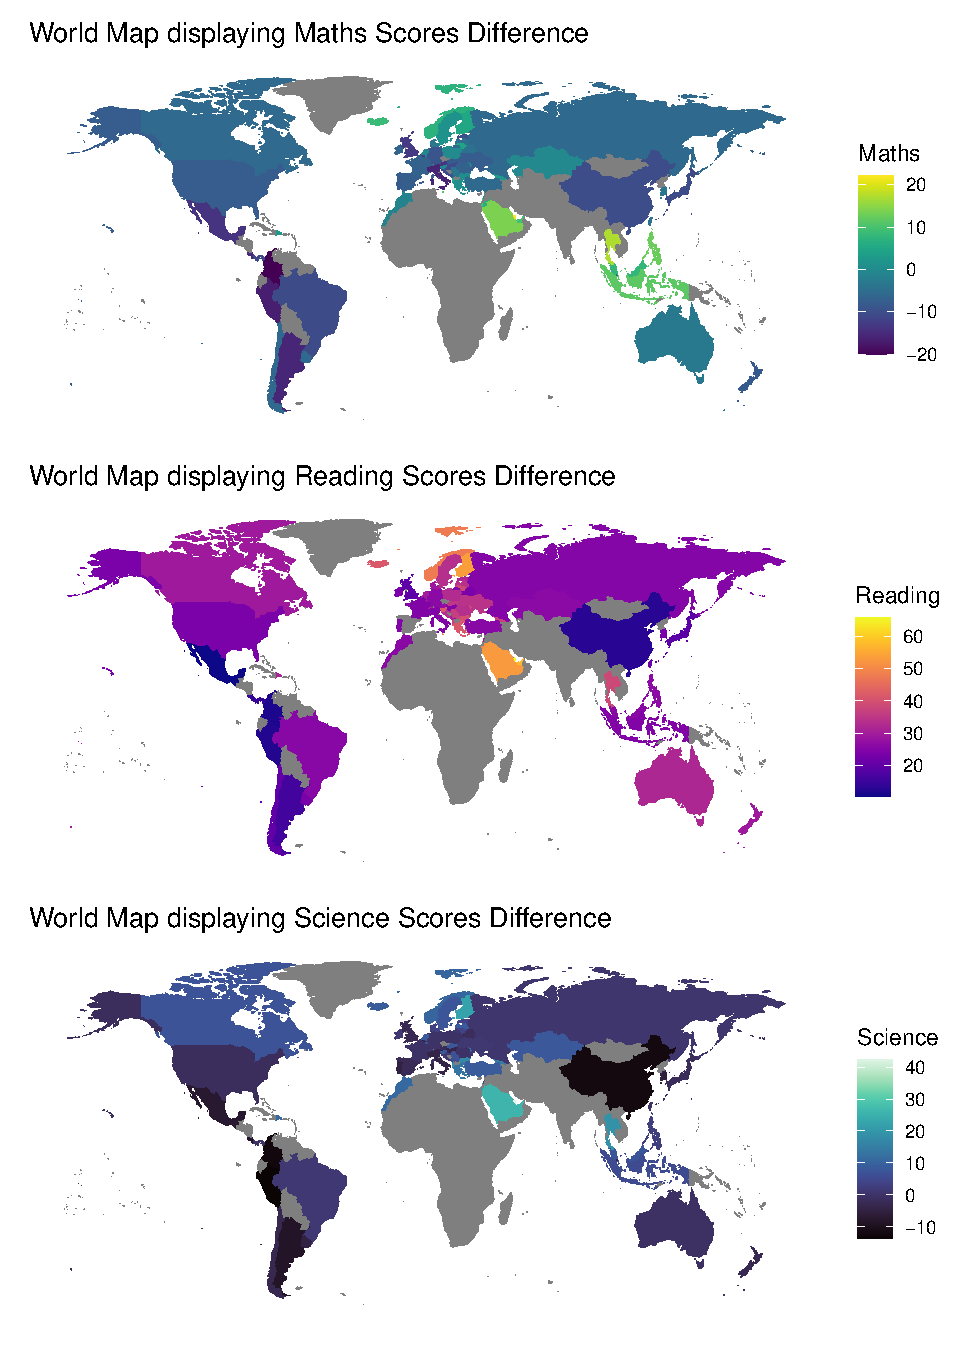
\includegraphics[width=1\linewidth]{learningtower_files/figure-latex/ggplot-maps-1} \caption[Maps]{Maps}\label{fig:ggplot-maps}
\end{figure}
\end{Schunk}

Figure \ref{fig:ggplot-maps}

\hypertarget{socioeconomic-factors-analysis}{%
\section{Socioeconomic Factors
Analysis}\label{socioeconomic-factors-analysis}}

\hypertarget{corr-plot}{%
\subsection{Corr plot}\label{corr-plot}}

\begin{Schunk}
\begin{figure}[H]
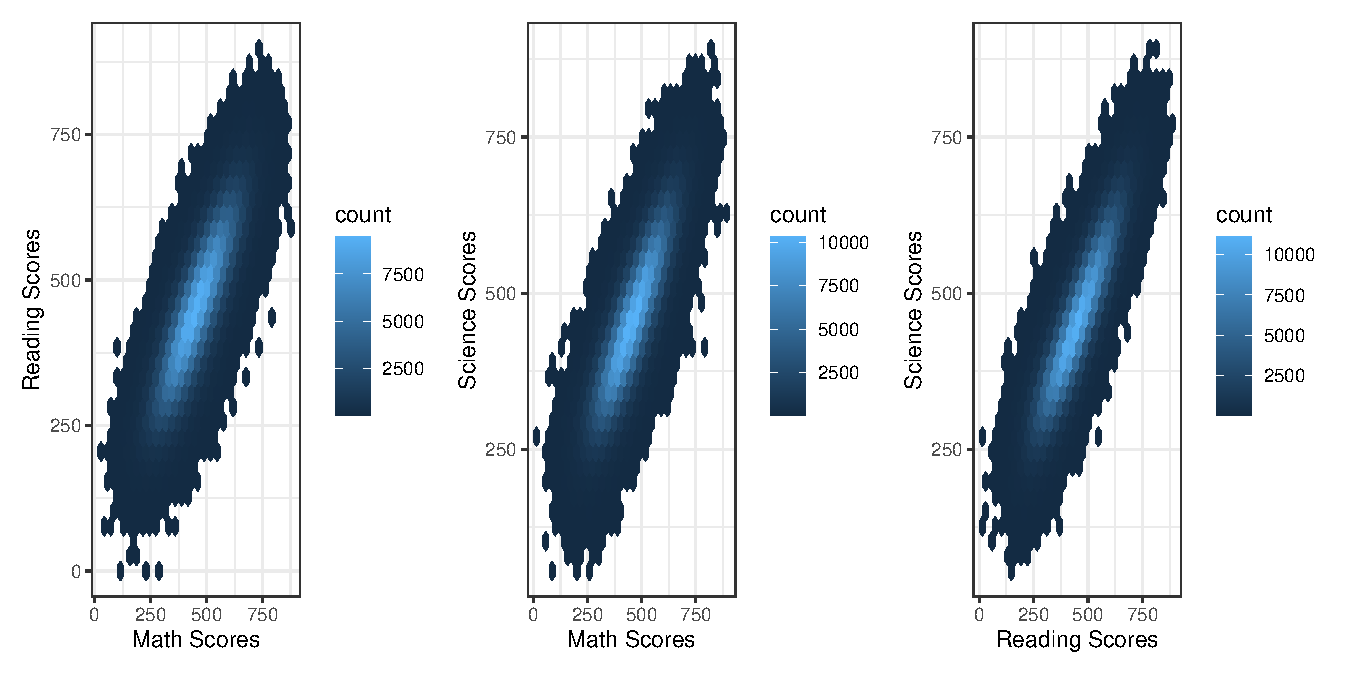
\includegraphics[width=1\linewidth]{learningtower_files/figure-latex/corr-plot-1} \caption[Correlation Plot]{Correlation Plot}\label{fig:corr-plot}
\end{figure}
\end{Schunk}

Figure \ref{fig:corr-plot}

\hypertarget{qual-plot}{%
\subsection{Qual Plot}\label{qual-plot}}

\begin{Schunk}
\begin{figure}[H]
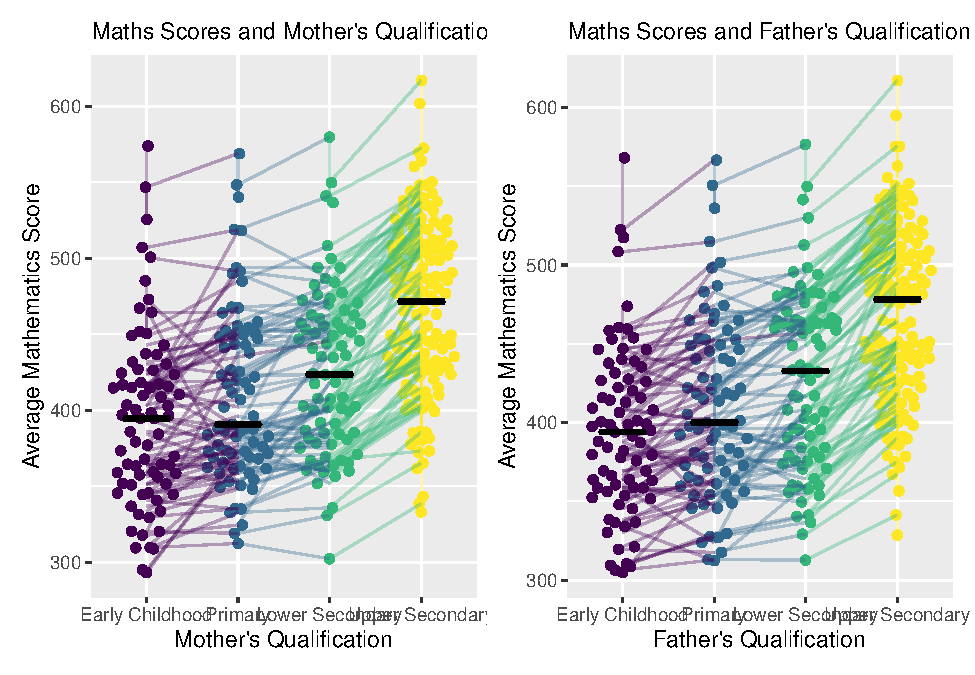
\includegraphics[width=1\linewidth]{learningtower_files/figure-latex/qual-plot-1} \caption[Qualification Plots]{Qualification Plots}\label{fig:qual-plot}
\end{figure}
\end{Schunk}

Figure @\ref(fig:qual-plot)

\hypertarget{tv-plots}{%
\subsection{TV Plots}\label{tv-plots}}

\hypertarget{temoral-trend-australia}{%
\section{Temoral Trend Australia}\label{temoral-trend-australia}}

\bibliography{learningtower.bib}

\address{%
Priya Ravindra Dingorkar\\
Monash University\\%
Department Econometrics and Business Statistics\\ Clayton, Australia\\
%
\url{https://www.linkedin.com/in/priya-dingorkar/}\\%
%
\href{mailto:priyadingorkar@gmail.com}{\nolinkurl{priyadingorkar@gmail.com}}%
}

\address{%
Kevin Y.X. Wang\\
University of Sydney\\%
Data scientist\\ Illumina, Inc.\\ School of Mathematics and
Statistics\\ Sydney, Australia\\
%
\url{https://kevinwang09.github.io/}\\%
%
\href{mailto:kevinwangstats@gmail.com}{\nolinkurl{kevinwangstats@gmail.com}}%
}

\address{%
Dianne Cook\\
Monash University\\%
Department Econometrics and Business Statistics\\ Clayton, Australia\\
%
\url{http://dicook.org/}\\%
%
\href{mailto:dicook@monash.edu}{\nolinkurl{dicook@monash.edu}}%
}
